\chapter{Results and Discussions}
The chapter is organized as follows: Section \ref{sec:ch4_desc_stat} will discuss the result of the descriptive statistics; Section \ref{sec:ch4_morphological_analysis} will discuss the results on morphological analysis; Section \ref{sec:ch4_structural_analysis} will discuss the structural analysis including the Mathematical structures of the Qur'\=an. Section \ref{sec:ch4_topic_modeling_result} will discuss the results for thematic analysis using both statistical and Large Language models. Further, 
Section \ref{sec:ir_result} will discuss the Information Retrieval result.
\section{Descriptive Statistics}\label{sec:ch4_desc_stat}
In this section, the count statistics for the verses and words of the Qur'an. Figure \ref{fig:ayah_word_count} shows the count of \arb[trans]{ayAt} \arb{ayAt} (verses) and word of the Qur'an.

\begin{figure}[!b]
    \centering
    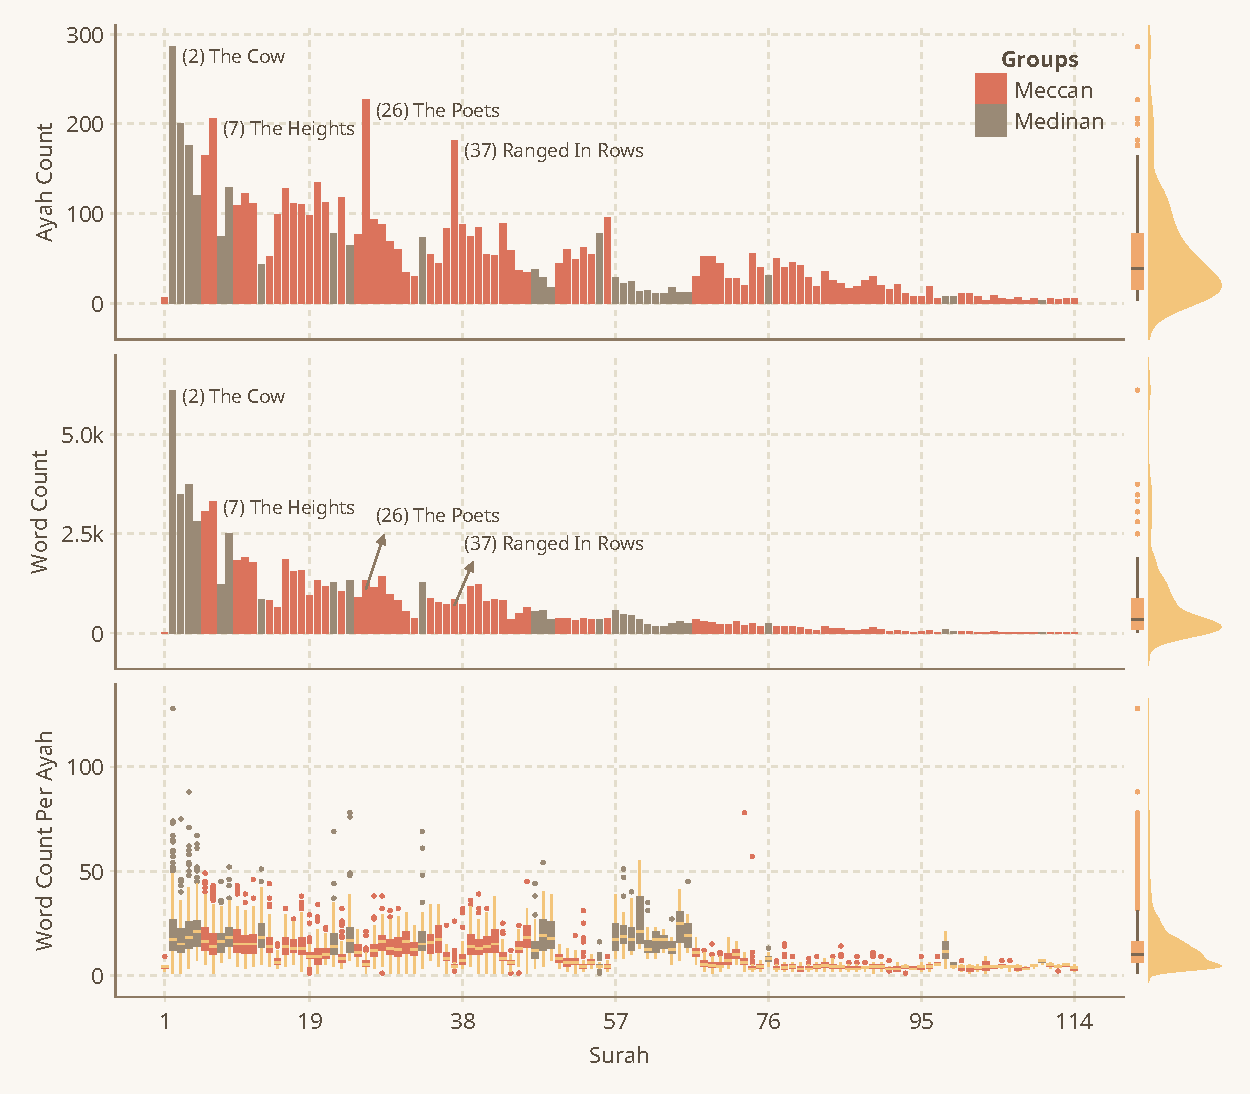
\includegraphics[width=\textwidth]{img/plot1.pdf}
    \caption{Statistics of the words and \arb[trans]{ayAt} \arb{ayAt} (verses) of the Qur'\=an}
    \label{fig:ch4_ayah_word_count}
\end{figure}

\begin{figure}[!b]
    \centering
    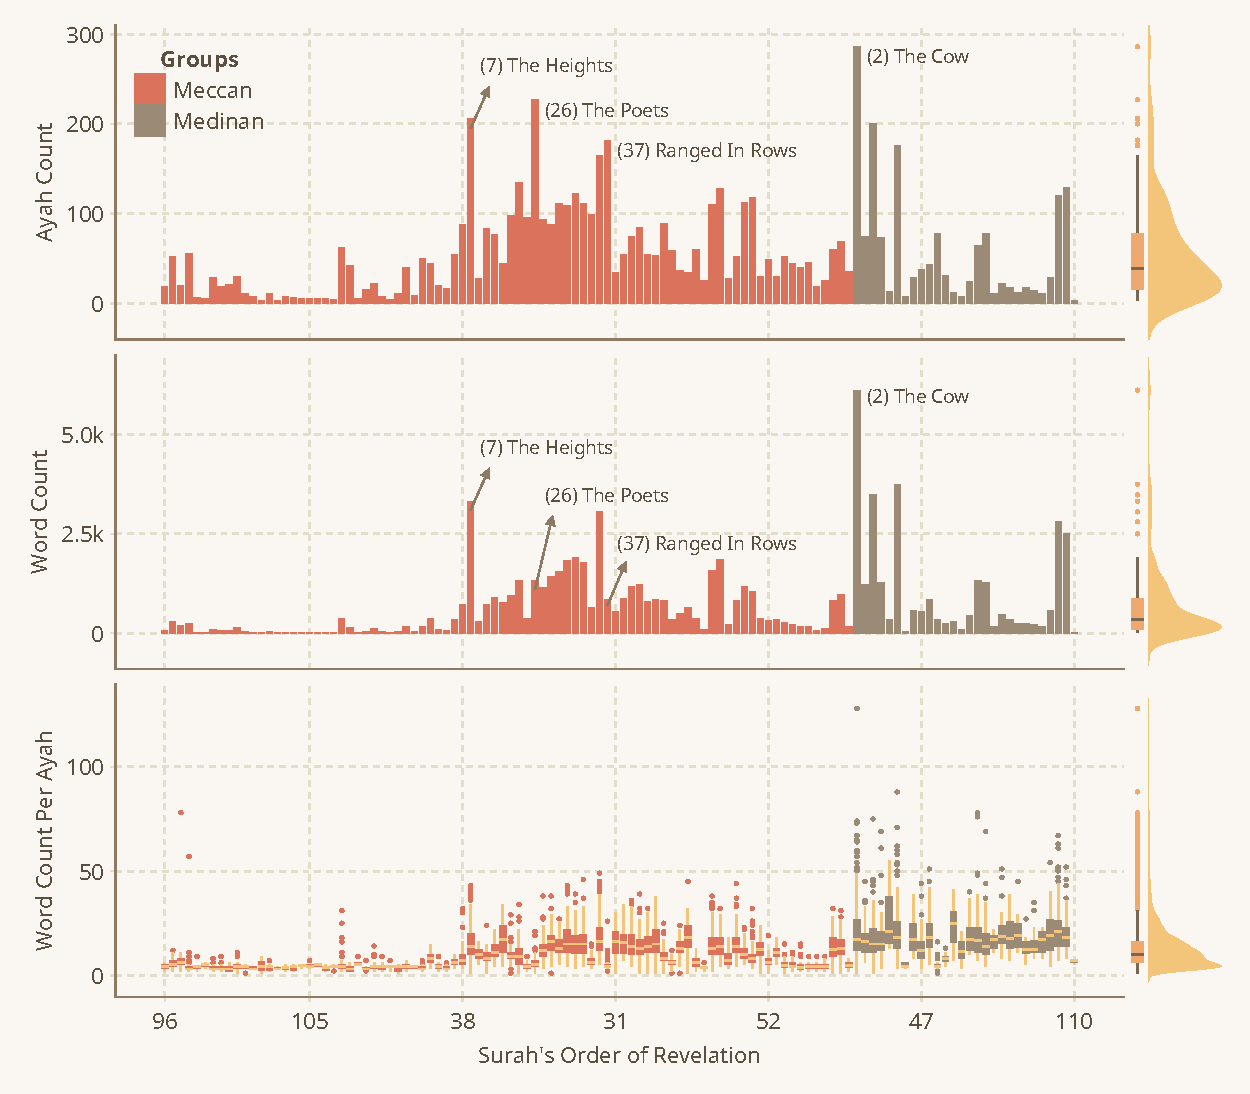
\includegraphics[width=\textwidth]{img/plot2.pdf}
    \caption{Statistics of the words and \arb[trans]{ayAt} \arb{ayAt} (verses) of the Qur'\=an according to revelation order}
    \label{fig:ch4_ayah_word_count_rev_order}
\end{figure}

\subsection{Verses}\label{sec:ch4_desc_stat_verse}
\section{Morphological Analysis}\label{sec:ch4_morphological_analysis}
\section{Structural Analysis}\label{sec:ch4_structural_analysis}
\subsection{Concentric Structure}
\subsection{Mathematical Structure}
\subsection{Discussions on Islamic Philosophy of Qur'\=an's Structural Analysis}
\section{Topic Modeling}\label{sec:ch4_topic_modeling_result}
\subsection{Latent Dirichlet Allocation}
\subsection{Bidirectional Encoder Representation from Transformer}
\subsection{Generative Pre-Trained Transformer}
\section{Relating to other Islamic Texts and Analyses}
\subsection{Retrieval-Augmented Generation Approach}
\section{Limitations of the Models}
\label{sec:ch4_ir_result}


